\section{$\rho_2$ cannot be a 4-transposition}

\paragraph{}
By Lemma~\ref{min-4-trans}, at least one 4-transposition is needed. It can neither be at position $\rho_0$ by Lemma~\ref{exclude-0} nor in position $\rho_1$ by Theorem~\ref{exclude-1} therefore, $\rho_2$ must be the 4-transposition.

\paragraph{}
In the Theorem~\ref{find-2} we will use the method defined in~\ref{find-2} to find some sggis. In this case none of the generators of a sggi can be written as a product of the other. The permutation representation graph of those sggis are displayed in appendix~\ref{monodromy-5}. After that we will prove in Theorem~\ref{exclude-2} that none of those sggis satisfies the intersection property and thus none of them are string C-groups.

\begin{theorem}
  \label{find-2}
  The only permutation representation graph of rank 5 on 11 points are those displayed in appendix~\ref{monodromy-5} (p.~\pageref{monodromy-5}).
\end{theorem}

\begin{proof}
  In this case, we will start with the $\rho_2$ 4-transposition.

  \begin{figure}[H]
    \begin{center}
      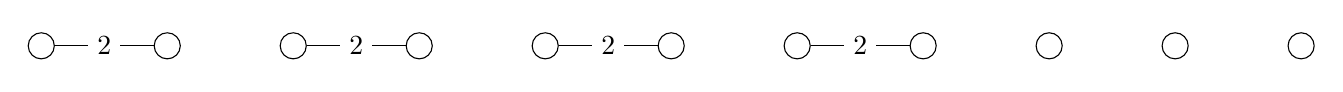
\begin{tikzpicture}[scale=.8]

        \begin{scope}[every node/.style={circle,draw}]
          \node (1)  at (-2,0)  {};
          \node (2)  at (0,0)  {};
          \node (3)  at (2,0)  {};
          \node (4)  at (4,0)  {};
          \node (5)  at (6,0)  {};
          \node (6)  at (8,0)  {};
          \node (7)  at (10,0)  {};
          \node (8)  at (12,0)  {};
          \node (9)  at (14,0)  {};
          \node (10)  at (16,0)  {};
          \node (11)  at (18,0)  {};
        \end{scope}

        \begin{scope}[every node/.style={fill=white}]

          \begin{scope}[every edge/.style={draw}]
            \path (1)  edge node {$2$} (2);
            \path (3)  edge node {$2$} (4);
            \path (5)  edge node {$2$} (6);
            \path (7)  edge node {$2$} (8);
          \end{scope}
        \end{scope}

      \end{tikzpicture}
      \caption{}
    \end{center}
  \end{figure}

\paragraph{}
The involutions $\rho_0$ and $\rho_4$ must commute with $\rho_2$ thus when adding their edges to the graph, only the patterns saw in~\ref{patterns-adding} are possible. But $\rho_0$ and $\rho_4$ must commute too. Thus they must form patterns saw in~\ref{intersection-patterns}.

\paragraph{}
Since there is only one 4-transposition, there are only 12 edges available to link 11 points, 2 more than the minimum. Thus if a edge is added, it must link two distinct components, expect two times. Those two edges are called "joker" edges. When an alternating square is built, one of those edge is used, it is the same if a double edge is built.

\paragraph{}
A choice must be made among the three possibilities for each involution. We will prove that one involution must form an alternating square and that the other must make a double edge and link two fixed point of $\rho_2$.

\paragraph{}
First, we will prove that none of the involutions can make two double edges. Then we will prove that the same pattern cannot be used for both involutions.

\paragraph{}
Each pattern of Lemma~\ref{patterns-adding} use at least one edge. Thus none of the patterns that we will use can us both "joker" edges and leaves nothing to the other involution. Therefore the pattern consisting of two double edges is impossible.

\paragraph{}
Now we will prove the both patterns cannot build one double edge on link two fixed points at the same time. There is only three points fixed by $\rho_2$. If both involutions choose to make one alternating square and link two fixed points they must share at least one of the fixed points. Then a $\rho_0$ and a $\rho_4$ edge will share a vertex but that is forbidden by Lemma~\ref{0-4-no-share}.

\paragraph{}
If both involutions make an alternating square with $\rho_2$ there are two possibilities: the two squares can share some vertices or none.


\paragraph{}
If they share some vertices then a $\rho_0$ and a $\rho_4$ involution will share a vertex but that is forbidden by Lemma~\ref{0-4-no-share}.

\paragraph{}
If the two squares does not share a vertex, the graph is the following.

\begin{figure}[H]
  \begin{center}
    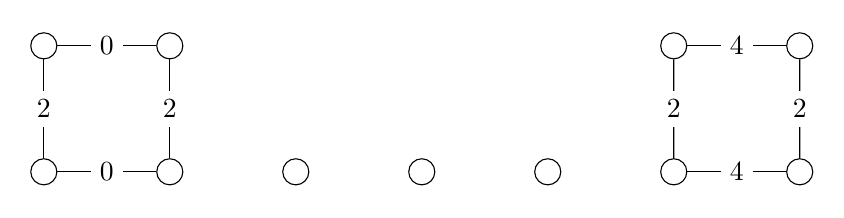
\begin{tikzpicture}[scale=.8]

      \begin{scope}[every node/.style={circle,draw}]
        \node (1)  at (0,0)  {};
        \node (2)  at (0,2)  {};
        \node (3)  at (2,0)  {};
        \node (4)  at (2,2)  {};
        \node (5)  at (4,0)  {};
        \node (6)  at (6,0)  {};
        \node (7)  at (8,0)  {};
        \node (8)  at (10,0)  {};
        \node (9)  at (10,2)  {};
        \node (10)  at (12,0)  {};
        \node (11)  at (12,2)  {};
      \end{scope}

      \begin{scope}[every node/.style={fill=white}]

        \begin{scope}[every edge/.style={draw}]
          \path (1)  edge node {$0$} (3);
          \path (2)  edge node {$0$} (4);
          \path (1)  edge node {$2$} (2);
          \path (3)  edge node {$2$} (4);
          \path (8)  edge node {$2$} (9);
          \path (10) edge node {$2$} (11);
          \path (8)  edge node {$4$} (10);
          \path (9)  edge node {$4$} (11);
        \end{scope}
      \end{scope}

    \end{tikzpicture}
    \caption{}
  \end{center}
\end{figure}

\paragraph{}
All "joker" edges have been used so no more alternating square can be built. But the left square must be connected by a $\rho_1$ edge and the right one by a $\rho_3$ edge. We need to find a chain that connect the left square to the right square with only $\rho_1$ and $\rho_3$ edges. But that is impossible because the indices must be consecutive in a chain by Lemma~\ref{chain-consecutive}.

\paragraph{}
Therefore one of the involution must build an alternating square and the other must build a double edge and link two fixed points. By duality, only the case where $\rho_4$ makes an alternating square will be considered and the other makes a double edge and links two fixed points.

\begin{figure}[H]
  \begin{center}
    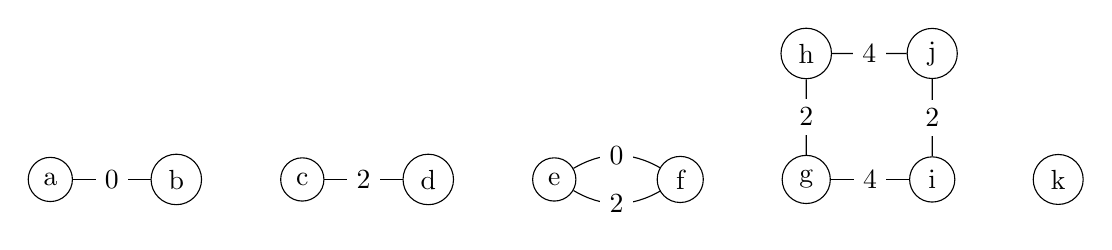
\begin{tikzpicture}[scale=.8]

      \begin{scope}[every node/.style={circle,draw}]
        \node (1)  at (12,2)  {h};
        \node (2)  at (12,0)  {g};
        \node (3)  at (14,2)  {j};
        \node (4)  at (14,0)  {i};
        \node (5)  at (6,0)  {d};
        \node (6)  at (4,0)  {c};
        \node (7)  at (10,0)  {f};
        \node (8)  at (8,0)  {e};
        \node (9)  at (2,0)  {b};
        \node (10) at (0,0)  {a};
        \node (11) at (16,0) {k};
      \end{scope}

      \begin{scope}[every node/.style={fill=white}]

        \begin{scope}[every edge/.style={draw}]
          \path (9)  edge node {$0$} (10);
          \path (7)  edge[bend right=30] node {$0$} (8);
          \path (1)  edge node {$2$} (2);
          \path (3)  edge node {$2$} (4);
          \path (5)  edge node {$2$} (6);
          \path (7)  edge[bend left=30] node {$2$} (8);
          \path (1)  edge node {$4$} (3);
          \path (2)  edge node {$4$} (4);
        \end{scope}
      \end{scope}

    \end{tikzpicture}
    \caption{The graph with $\rho_0$, $\rho_2$ and $\rho_4$}
  \end{center}
\end{figure}

\paragraph{}
Now that all of our "joker" edges has been used, every other edge must link two different connected components of the graph.

\paragraph{}
Now the $\rho_3$ edge will be placed. It cannot be adjacent to the component $\{a,b\}$ or $\{e,f\}$ by Proposition~\ref{chain-consecutive} and~\ref{adjacent-double} respectively. There are three components that can be connected by two $\rho_3$ edges.After placing all $\rho_3$ edges, those three component will form one big component. Then the $\rho_1$ edges will be placed and they must be able to connect to this new component. But the edge $(c,d)$ is only component from the three that can be connected to a $\rho_1$ edge. Therefore one end of this edge must remain free.

\paragraph{}
The fixed point cannot be connected twice by $\rho_3$ edges by Proposition~\ref{fixed-only-1}. So there is only one possibility. One edge must connect the component $\{e,f\}$ to the component $\{g,h,i,j\}$ and the other must connect $\{g,h,i,j\}$ to the fixed point $k$.

\paragraph{}
The square must thus be connected twice. There are three possibilities: the two connected vertices can be opposed or adjacent and, in this case, separated by a $\rho_1$ or a $\rho_3$ edge. This does not influence the position of the $\rho_1$ edges. It is possible to continue building the graph without having to deal with cases. Here is one of the possible graphs:

\begin{figure}[H]
  \begin{center}
    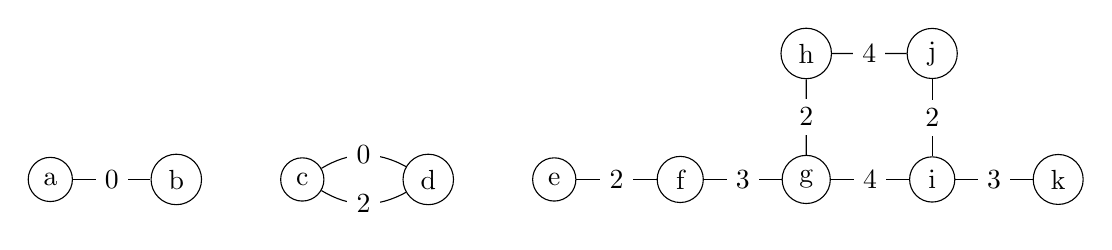
\begin{tikzpicture}[scale=.8]

      \begin{scope}[every node/.style={circle,draw}]
        \node (1)  at (0,2)  {j};
        \node (2)  at (0,0)  {i};
        \node (3)  at (-2,2)  {h};
        \node (4)  at (-2,0)  {g};
        \node (5)  at (-6,0)  {e};
        \node (6)  at (-4,0)  {f};
        \node (7)  at (-10,0)  {c};
        \node (8)  at (-8,0)  {d};
        \node (9)  at (-14,0)  {a};
        \node (10) at (-12,0)  {b};
        \node (11) at (2,0) {k};
      \end{scope}

      \begin{scope}[every node/.style={fill=white}]

        \begin{scope}[every edge/.style={draw}]
          \path (9)  edge node {$0$} (10);
          \path (7)  edge[bend left=30] node {$0$} (8);
          \path (1)  edge node {$2$} (2);
          \path (3)  edge node {$2$} (4);
          \path (5)  edge node {$2$} (6);
          \path (7)  edge[bend right=30] node {$2$} (8);
          \path (2)  edge node {$3$} (11);
          \path (4)  edge node {$3$} (6);
          \path (1)  edge node {$4$} (3);
          \path (2)  edge node {$4$} (4);
        \end{scope}
      \end{scope}

    \end{tikzpicture}
    \caption{One of the graphs after placing $\rho_3$ edges}
  \end{center}
\end{figure}

\paragraph{}
Now the two edges of $\rho_1$ must be placed. A $\rho_1$ edge must link the component $\{a,b\}$ and $\{c,d\}$. Due to the symmetry, the choice of the points does not change anything. We will choose to link $b$ and $c$.

\begin{figure}[H]
  \begin{center}
    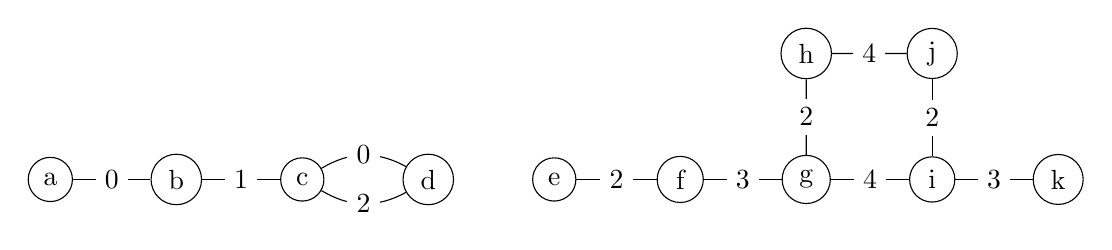
\begin{tikzpicture}[scale=.8]

      \begin{scope}[every node/.style={circle,draw}]
        \node (1)  at (0,2)  {j};
        \node (2)  at (0,0)  {i};
        \node (3)  at (-2,2)  {h};
        \node (4)  at (-2,0)  {g};
        \node (5)  at (-6,0)  {e};
        \node (6)  at (-4,0)  {f};
        \node (7)  at (-10,0)  {c};
        \node (8)  at (-8,0)  {d};
        \node (9)  at (-14,0)  {a};
        \node (10) at (-12,0)  {b};
        \node (11) at (2,0) {k};
      \end{scope}

      \begin{scope}[every node/.style={fill=white}]

        \begin{scope}[every edge/.style={draw}]
          \path (9)  edge node {$0$} (10);
          \path (7)  edge[bend left=30] node {$0$} (8);
          \path (10) edge node {$1$} (7);
          \path (1)  edge node {$2$} (2);
          \path (3)  edge node {$2$} (4);
          \path (5)  edge node {$2$} (6);
          \path (7)  edge[bend right=30] node {$2$} (8);
          \path (2)  edge node {$3$} (11);
          \path (4)  edge node {$3$} (6);
          \path (1)  edge node {$4$} (3);
          \path (2)  edge node {$4$} (4);
        \end{scope}
      \end{scope}

    \end{tikzpicture}
    \caption{}
  \end{center}
\end{figure}


\paragraph{}
The component $\{e,f,g,h,i,j,k\}$ must be linked by $e$ as explained above. For the component $\{a,b,c,d\}$ there are two possibilities: $a$ or $d$. Both solutions create a valid sggis graph. Here is one of the graphs:

\begin{figure}[H]
  \begin{center}
    \begin{tikzpicture}[scale=.8]

      \begin{scope}[every node/.style={circle,draw}]
        \node (1)  at (0,2)  {};
        \node (2)  at (0,0)  {};
        \node (3)  at (-2,2)  {};
        \node (4)  at (-2,0)  {};
        \node (5)  at (-6,0)  {};
        \node (6)  at (-4,0)  {};
        \node (7)  at (-10,0)  {};
        \node (8)  at (-8,0)  {};
        \node (9)  at (-14,0)  {};
        \node (10) at (-12,0)  {};
        \node (11) at (2,0) {};
      \end{scope}

      \begin{scope}[every node/.style={fill=white}]

        \begin{scope}[every edge/.style={draw}]
          \path (9)  edge node {$0$} (10);
          \path (7)  edge[bend left=30] node {$0$} (8);
          \path (5)  edge node {$1$} (8);
          \path (7)  edge node {$1$} (10);
          \path (1)  edge node {$2$} (2);
          \path (3)  edge node {$2$} (4);
          \path (5)  edge node {$2$} (6);
          \path (7)  edge[bend right=30] node {$2$} (8);
          \path (2)  edge node {$3$} (11);
          \path (4)  edge node {$3$} (6);
          \path (1)  edge node {$4$} (3);
          \path (2)  edge node {$4$} (4);
        \end{scope}
      \end{scope}

    \end{tikzpicture}
    \caption{One sggi on $A_{11}$ of rank 5}
  \end{center}
\end{figure}

\paragraph{}
When placing the $\rho_3$ edge we made a choice between three possibilities, for the $\rho_1$ edge it was among two possibilities. Thus in total the are 6 graphs. The construction of the five other graphs is left to the reader. He can check that the graphs built match the graphs of appendix~\ref{monodromy-5}.

\end{proof}


\begin{theorem}
  \label{exclude-2}
  None of the groups represented by the graphs of appendix~\ref{monodromy-5} are C-groups.
\end{theorem}

\begin{proof}
  By the definition of a C-group, it is sufficient to find two subsets of generators $S_1$ and $S_2$ such that $\Gamma_{S_1} \cap \Gamma_{S_2} \neq \Gamma_{S_1 \cap S_2}$.

  \paragraph{}
  This proof is inspired by the section 4 of~\cite{leemansTransactions}.

  \paragraph{}
  In this case, they will be choose $S_1 = \{\rho_1, \rho_2\}$ and $S_2 = \{\rho_2, \rho_3, \rho_4\}$. Here $S_1 \cap S_2 = \{\rho_2\}$ and so $\Gamma_{S_1 \cap S_2} = \Gamma_{\rho_2}$ is a cyclic group of order 2. Hence, $\rho_2$ is an involution.

  \paragraph{}
  $S_1$ will be studied more deeply, only the $\rho_1$ and $\rho_2$ edges are kept in all the possible graphs. There are only two possible graphs:

  \begin{figure}[H]
    \begin{center}
      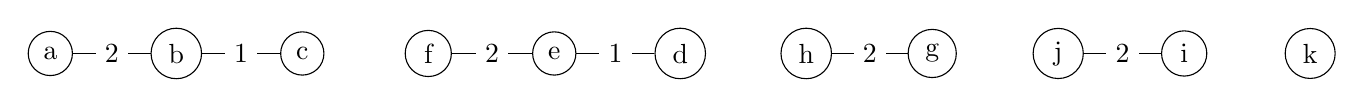
\begin{tikzpicture}[scale=.8]

        \begin{scope}[every node/.style={circle,draw}]
          \node (1)  at (-2,0)  {a};
          \node (2)  at (0,0)  {b};
          \node (3)  at (2,0)  {c};
          \node (4)  at (8,0)  {d};
          \node (5)  at (6,0)  {e};
          \node (6)  at (4,0)  {f};
          \node (7)  at (12,0)  {g};
          \node (8)  at (10,0)  {h};
          \node (9)  at (16,0)  {i};
          \node (10) at (14,0)  {j};
          \node (11)  at (18,0)  {k};
        \end{scope}

        \begin{scope}[every node/.style={fill=white}]

          \begin{scope}[every edge/.style={draw}]
            \path (2)  edge node {$1$} (3);
            \path (4)  edge node {$1$} (5);
            \path (1)  edge node {$2$} (2);
            \path (5)  edge node {$2$} (6);
            \path (7)  edge node {$2$} (8);
            \path (9)  edge node {$2$} (10);
          \end{scope}
        \end{scope}

      \end{tikzpicture}
      \caption{First possibility for $\Gamma_{S_1}$}
    \end{center}
  \end{figure}

  \begin{figure}[H]
    \begin{center}
      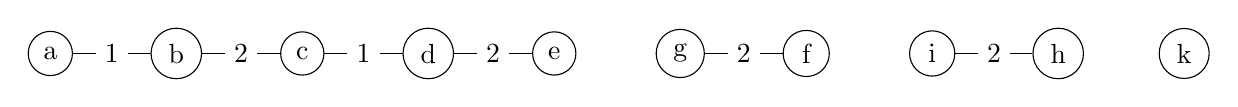
\begin{tikzpicture}[scale=.8]

        \begin{scope}[every node/.style={circle,draw}]
          \node (2)  at (0,0)  {a};
          \node (3)  at (2,0)  {b};
          \node (4)  at (4,0)  {c};
          \node (5)  at (6,0)  {d};
          \node (6)  at (8,0)  {e};
          \node (7)  at (12,0)  {f};
          \node (8)  at (10,0)  {g};
          \node (9)  at (16,0)  {h};
          \node (10) at (14,0)  {i};
          \node (1)  at (18,0)  {k};
        \end{scope}

        \begin{scope}[every node/.style={fill=white}]

          \begin{scope}[every edge/.style={draw}]
            \path (2)  edge node {$1$} (3);
            \path (4)  edge node {$1$} (5);
            \path (3)  edge node {$2$} (4);
            \path (5)  edge node {$2$} (6);
            \path (7)  edge node {$2$} (8);
            \path (9)  edge node {$2$} (10);
          \end{scope}
        \end{scope}

      \end{tikzpicture}
      \caption{Second possibility for $\Gamma_{S_1}$}
    \end{center}
  \end{figure}

  \paragraph{}
  In the first graph, the permutation $(\rho_1 \rho_2)^2 \rho_1$ is $(a~b)(d~e)$. Thus this permutation permutes only 4 out of the 8 points of $\rho_2$.

  \paragraph{}
  In the second graph, $(\rho_1\rho_2)^4 \rho_1 = (b~c)(d~e)$ gives the same result.

  \paragraph{}
  Now, let's study $S_2$, the disposition of the edges alongside the alternating square is very important. Therefore there are 3 possibilities:

  \begin{figure}[H]
    \begin{center}
      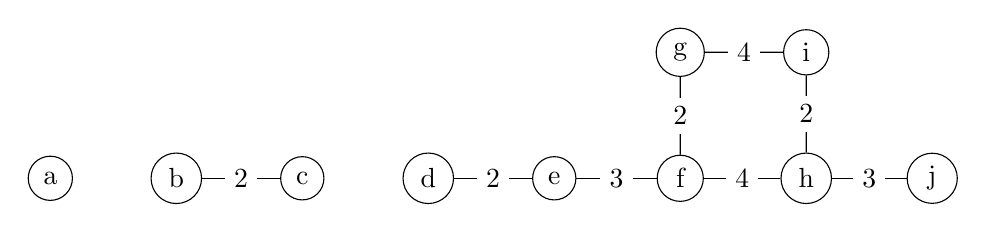
\begin{tikzpicture}[scale=.8]

        \begin{scope}[every node/.style={circle,draw}]
          \node (0)  at (-4,0)  {a};
          \node (1)  at (-2,0)  {b};
          \node (2)  at (0,0)  {c};
          \node (5)  at (2,0)  {d};
          \node (6)  at (4,0)  {e};
          \node (7)  at (6,0)  {f};
          \node (8)  at (6,2)  {g};
          \node (9)  at (8,2)  {i};
          \node (10) at (8,0)  {h};
          \node (11) at (10,0) {j};
        \end{scope}

        \begin{scope}[every node/.style={fill=white}]

          \begin{scope}[every edge/.style={draw}]
            \path (1)  edge node {$2$} (2);
            \path (5)  edge node {$2$} (6);
            \path (7)  edge node {$2$} (8);
            \path (9)  edge node {$2$} (10);
            \path (6)  edge node {$3$} (7);
            \path (10) edge node {$3$} (11);
            \path (7)  edge node {$4$} (10);
            \path (8)  edge node {$4$} (9);
          \end{scope}
        \end{scope}

      \end{tikzpicture}
      \caption{First possibility for $\Gamma_{S_2}$}
      \label{S2-1}
    \end{center}
  \end{figure}

  \begin{figure}[H]
    \begin{center}
      \begin{tikzpicture}[scale=.8]

        \begin{scope}[every node/.style={circle,draw}]
          \node (0)  at (-4,0)  {};
          \node (1)  at (-2,0)  {};
          \node (2)  at (0,0)  {};
          \node (5)  at (2,0)  {};
          \node (6)  at (4,0)  {};
          \node (7)  at (6,0)  {};
          \node (8)  at (6,2)  {};
          \node (9)  at (8,0)  {};
          \node (10) at (8,2)  {};
          \node (11) at (10,2) {};
        \end{scope}

        \begin{scope}[every node/.style={fill=white}]

          \begin{scope}[every edge/.style={draw}]
            \path (1)  edge node {$2$} (2);
            \path (5)  edge node {$2$} (6);
            \path (7)  edge node {$2$} (8);
            \path (9)  edge node {$2$} (10);
            \path (6)  edge node {$3$} (7);
            \path (10) edge node {$3$} (11);
            \path (7)  edge node {$4$} (9);
            \path (8)  edge node {$4$} (10);
          \end{scope}
        \end{scope}

      \end{tikzpicture}
      \caption{Second possibility for $\Gamma_{S_2}$}
    \end{center}
  \end{figure}

  \begin{figure}[H]
    \begin{center}
      \begin{tikzpicture}[scale=.8]

        \begin{scope}[every node/.style={circle,draw}]
          \node (0)  at (-4,0)  {};
          \node (1)  at (-2,0)  {};
          \node (2)  at (0,0)  {};
          \node (5)  at (2,0)  {};
          \node (6)  at (4,0)  {};
          \node (7)  at (8,2)  {};
          \node (8)  at (6,2)  {};
          \node (9)  at (6,0)  {};
          \node (10) at (8,0)  {};
          \node (11) at (10,0) {};
        \end{scope}

        \begin{scope}[every node/.style={fill=white}]

          \begin{scope}[every edge/.style={draw}]
            \path (1)  edge node {$2$} (2);
            \path (5)  edge node {$2$} (6);
            \path (7)  edge node {$2$} (8);
            \path (9)  edge node {$2$} (10);
            \path (6)  edge node {$3$} (9);
            \path (10) edge node {$3$} (11);
            \path (7)  edge node {$4$} (10);
            \path (8)  edge node {$4$} (9);
          \end{scope}
        \end{scope}

      \end{tikzpicture}
      \caption{Third possibility for $\Gamma_{S_2}$}
    \end{center}
  \end{figure}

  \paragraph{}
  We will only do the graph displayed in Figure~\ref{S2-1}. The proof is similar for the two other graphs and is left to the reader.

  \paragraph{}
  We will prove that the $\Gamma_{\rho_2,\rho_3,\rho_4}$ is $S_7$ on the component $d,e,f,g,h,i,j$. To do this, we will first prove that the group is 2-transitive. Thus by Property~\ref{2-transitive-primitive}, it is primitive. But the primitive group are well-known and the list of all primitive groups of degree less than 50 is available in~\cite{buekenhout1996list}.

  \paragraph{}
  The group is transitive because its graph is connected. To prove that the group is 2-transitive we will use Property~\ref{practical-transitivity}. We try to find a permutation that send $i$ to any other point while keeping $j$ fixed. If the permutation does not contains $\rho_3$ then $j$ is fixed. Thus in fact there are two orbits : $\{d,e\}$ and $\{f,g,h,i\}$. The vertex $i$ is already in the second orbit, thus it can be easily send to every other point of the orbit.

  \paragraph{}
  We need to find a permutation that send $i$ to $d$ or $e$ while keeping $j$ in place. The permutation $\rho_2 \rho_4 \rho_3 \rho_2 \rho_3 \rho_2 \rho_3$ is a solution that send $d$ to $e$. $\Gamma_{\rho_2, \rho_3, \rho_4}$ is 2-transitive and thus primitive on $\{d,e,f,g,h,i,j\}$

  \paragraph{}
  We will now look at the list of all primitive groups~\cite{buekenhout1996list}. We will compute the size of some subgroup. But by Property~\ref{magic-formula} the order of a group is a multiple of the size of its subgroups. Thus the order of the group must be an multiple of the least common multiple of the size of some subgroups.

  \paragraph{}
  The group is 2-transitive and so its order is a multiple of $7 \times 6 = 42$. $\Gamma_{\rho_2, \rho_3}$ is $D_{10}$ which is of order 10. Thus the order of the group must is a multiple of the least common divisor of 42 and 10 which is 240. But the only groups that satisfies this condition are $A_7$ and $S_7$. $\rho_2$ is an odd involution and cannot be member of $A_7$ thus the group must be $S_7$.

  \paragraph{}
  But then every $\rho_2$ edge is an involution on those seven points. Thus it is also possible to find a permutation that only move 4 points out of the 8 points of $\rho_2$. This permutation is in $\Gamma_{S_1}$ and in $\Gamma_{S_2}$ but not in $\Gamma_{\rho_2}$ thus $\Gamma$ does not satisfy the intersection property and is not a C-group.

\end{proof}

\paragraph{}
now

\begin{theorem}
  There does not exists a string C-group representation of rank 5 of $A_{11}$.
\end{theorem}

\paragraph{}
Now we have proven that there is no abstract polytopes of rank $5$ on $A_{11}$. Next we will prove the same for rank 4.
